\chapter{Algorithms}{}
\label{chap:algorithms}

\lettrine[lraise=0.1, nindent=0em, slope=-.5em]{N}{OW THAT THE POLICY} behind \uppercase{SNIPR} has been stated, the next step is to describe the problem the SNIPR's algorithms plan to solve.
% 
% In most programming settings, manually performing program transformations on a large collection of snippets is error prone and cumbersome, while programming solutions from scratch is often beyond the skill-set of most programmers. Consequently, it is more practical to use program transformation systems to take some of the burden of manually performing transformations off the developers.

Most code search approaches that use program transformations start with specifying automated program transformation procedures and parameterizing source code text fragments, and derive either: (1) hierarchical code generation rules~\cite{Nita:2010en} for runtime-code generation, (2) new or alternative program implementations~\cite{Wightman:2012gc}, or (3) domain specific languages for program adaptation~\cite{Visser:2001tc}.

While these outcomes have indeed proven successful, they still impose a significant manual effort on the developers---e.g., developers need to spend additional effort to make these solutions configurable and ready to go. Consequently, these methods are impractical if they are to be used---as is---in a \uppercase{SNIPR}-aware code search engine. 

The above observation is the motivation for the algorithms discussed in this chapter. The aim of these algorithms is to efficiently learn and use coherent mapping-based program transformations. By applying these transformations to a snippet, \uppercase{SnipR} can replace the structure of one snippet with the structure of another. The goal is for this to happen with minimal or no cost to the developer. 

Briefly, these algorithms represent the modules required to implement \uppercase{SnipR} functionality. For instance, the Setup step populates the \emph{Snippet Space} at indexing time, by invoking a code clone searching and detection tool. Then, the Learning step builds mappings for all the (original-clone) pairs in the \emph{Snippet Space}. When invoking \uppercase{SnipR}'s Twist (See Chapter~\ref{chap:twist} for details), the Matching step first maps the retargeting request to its corresponding optimal mapping and then applies the mapping to the original snippet.

In the reminder of this chapter, the algorithms or steps \uppercase{SnipR} needed to set-up and do code retargeting in a snippet-centric search engine are described in more detail. 

\section{The Setup Step}
\label{sec:precomputation}

This algorithm relies on the state-of-art approaches in code clone searching and detection~\cite{Jiang:2007cj, Roh:2010ts} in order to reveal, per an indexed snippet, a set of snippet alternatives (clones). These clones are needed to realize the way \uppercase{SnipR}'s learning algorithm operates. By definition, they are related implementations and thus similar. They are also syntactically different and are indeed \emph{interchangeable}. This knowledge is used by the learning algorithm to hypothesize and map together related code elements between snippets. 

This algorithm is based on the following intuition. Even though code clone searching and detection tools, called CSD from now on, might consider a tremendous space of alternative snippets for a single snippet, the number of unique snippet alternatives and therefore the number of snippet instances to use is much lower. Consequently, it makes sense to cache and reuse the set of unique alternative snippets computed by CSD, instead of performing multiple invocations only to compute the same snippets multiple times. The resulting set of (original-clone) pairs---$S = \{(s_1, s_2) x (s_1, s_3) x (s_1, s_4) ... x (s_1, s_n)\}$---will be saved in the \emph{Snippet Space} (cached snippets). This space, or the output of this algorithm, is computed by considering all the possible combinations of (original-clone) pairs that can be revealed by using an original snippet and its clones. The \emph{Snippet Space} is maintained in the same way indexes are maintained in a search engine.

For a larger number of libraries, the setup of a \emph{Snippet Space} becomes expensive, as a larger number of calls to CSD are required. To reduce this burden, the setup step builds the \emph{Snippet Space} incrementally, in-sync with the most popular libraries searched by users. By doing this, there is no need to consider all the possible combinations of (original-clone) pairs upfront; only a subset will be suffice.

\section{The Learning Step}
\label{sec:learning}

This section discusses, at a very high level, the learning algorithm for building mapping-based program transformations. These programming transformations allow \uppercase{SnipR} to transfer structure between similar code snippets; i.e., perform code retargeting. 

To learn code mappings in a principled way, we leverage techniques in structured prediction~\cite{Collins:2002uo}, which involve predicting objects with complex internal structure and dependencies---e.g., parse trees~\cite{Kumar:2011uj}. In particular, we cast the problem as a translation discovery problem: given a source and a clone snippet respectively, we induce a translation table over their similar structures. This table specify how two code snippets correspond. Once induced, this table can be used to determine structure translation candidates and thus synthesize a code mapping between the two snippets. 

The core of this algorithm is based on the hypothesis that a general code retargeting scheme can be produced by training a machine learning algorithm (machine learner) based on human-generated mappings (human-generated corpus). The machine learner can use the knowledge gained from the collected corpus to learn how to build mappings from further snippets using only what it learned during training. The entries of these mappings will specify how two related snippets correspond to one another (Figure~\ref{fig:mappings}). SNIPR uses these mappings to automate the process of changing the structure of one snippet to the structure of another. Mappings of this kind have an abstract syntax similar to the mapping syntax proposed by Nita and Notkin in their paper~\cite{Nita:2010en}.

\begin{figure}[!ht]
    \centering
    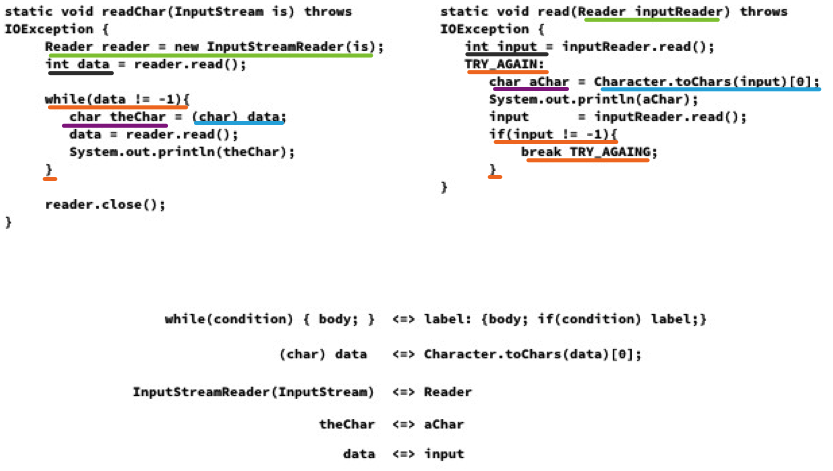
\includegraphics[width=\textwidth]{images/mappings}
    \caption{A simple mapping between two snippets.}
    \label{fig:mappings}
\end{figure}

Based on the above observation, the learning algorithm will use structured prediction---e.g., the generalized Perceptron~\cite{Collins:2002uo}---to learn how to write these code mappings. The corpus of human-generated mappings will be collected via a Web-based crowdsourcing application; the plan is to use either the Amazon's MechanicalTurk or a very basic Web application where users explicitly transform one snippet into another and map related code elements together. This information is used to train the machine learner.

In a nutshell, the learning algorithm takes as an input the \emph{Snippet Space}---computed by the setup step (See Section~\ref{sec:precomputation})---and a set of user constraints, such as data accessibility or function arity. These user constraints will help determine feasible regions, which are code areas where code retargeting can be applied. This algorithm will use syntactic analysis, in conjunction with these constraints, to help determine these areas. The feasibility of these areas is affected by different factors, such as the extent of local data declaration, control scope within functions, etc. Figure~\ref{fig:mappinggeneration} shows this process applied to a pair of snippets:

\begin{figure}[!ht]
    \centering
    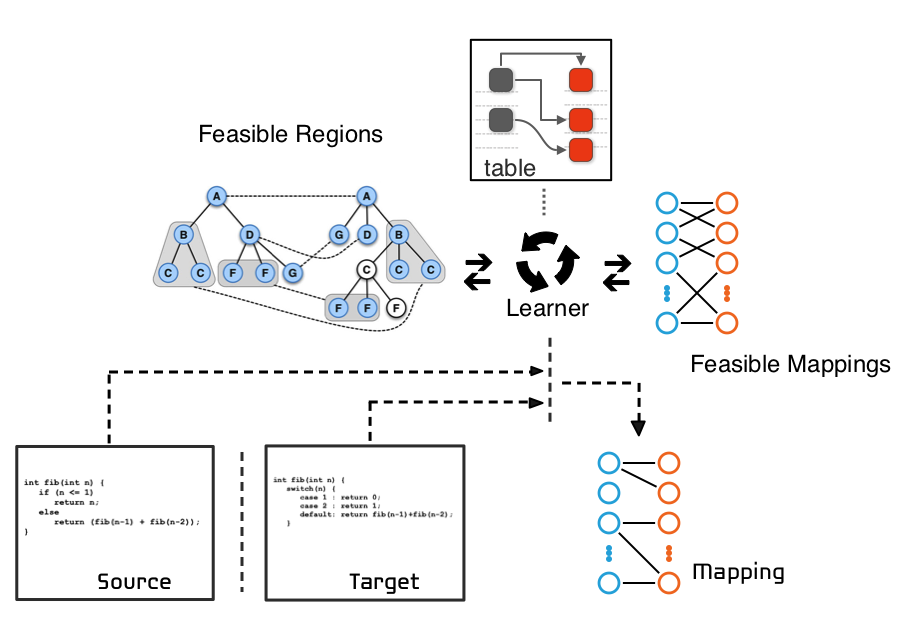
\includegraphics[width=\textwidth]{images/mappinggeneration}
    \caption{Learning a mapping-based transformation.}
    \label{fig:mappinggeneration}
\end{figure}

\section{The Matching Step}
\label{sec:matching}

This algorithm is responsible for determining the optimal mapping for a given retargeting request and applying it to a snippet implementation. \uppercase{SNIPR} will use a set of heuristics, in the form of a matching logic, that given a retargeting request, will efficiently assign the corresponding optimal mapping for each result. 

At a very high level, this algorithm takes as an input a query and a retargeting request (See Chapter~\ref{chap:twist}). Given this information, the matching step takes every mapping that explains the input. A variation of the explanatory power scheme, suggested in~\cite{Little:2008hr}, determines how well every mapping explains a sequence of tokens obtained from the input. This scheme states that tokens can be explained in numerous ways. One example could be a token that is matched with a function name is explained as invoking that function, and a token that is matched as part of a string is explained as helping create that string. Once the input is mapped to its corresponding optimal code mapping, the algorithm applies this code mapping to the original snippet implementation. This action produces a variation containing the changes specified by the mapping. Otherwise, it reports any found errors to the developer. 

This chapter has introduced the algorithms SNIPR uses to learn and use mapping-based program transformations in a code-centric search engine. To recap, these algorithms are the Setup Step, the Learning Step, and the Matching Step.
